\documentclass[11pt]{article}
\usepackage[hmargin=1in,vmargin=1in]{geometry}
\usepackage{xcolor}
\usepackage{amsmath,amssymb,amsfonts,url,sectsty,framed,tcolorbox,framed}
\newcommand{\pf}{{\bf Proof: }}
\newtheorem{theorem}{Theorem}
\newtheorem{lemma}{Lemma}
\newtheorem{proposition}{Proposition}
\newtheorem{definition}{Definition}
\newtheorem{remark}{Remark}
\newcommand{\qed}{\hfill \rule{2mm}{2mm}}
\newtheorem{example}{Example}
\usepackage{tikz}
\usepackage{bm}

\begin{document}
%%%%%%%%%%%%%%%%%%%%%%%%%%%%%%%%%%%%%%%%%%%%%%%%%%%%%%%%%%%%%%%%%%%%%
\noindent
\rule{\textwidth}{1pt}
\begin{center}
{\bf [CS304] Introduction to Cryptography and Network Security}
\end{center}
Course Instructor: Dr. Dibyendu Roy \hfill Winter 2023-2024\\
Scribed by: Raghav Agiwal (202151124) \hfill Lecture (Week 6)
\\
\rule{\textwidth}{1pt}
%%%%%%%%%%%%%%%%%%%%%%%%%%%%%%%%%%%%%%%%%%%%%%%s%%%%%%%%%%%%
%write here


\section{One Time Padding}
One Time Pad (OTP) in cryptography is a method of encrypting plaintext into ciphertext and decrypting ciphertext back into plaintext. It's based on the principle of exclusive OR (XOR) operation between the plaintext and a randomly generated secret key. The key must be as long as the plaintext and should never be reused for encrypting multiple messages
As we have discussed earlier, so we know encryption and decryption in OTP are given as:

\subsection{Encryption and Decryption}

\textbf{Encryption}: Ciphertext (C) is obtained by XORing the plaintext (M) with the secret key (K): \(C = M \oplus K\) \\
\textbf{Decryption}: Plaintext (M) is obtained by XORing the ciphertext (C) with the same secret key (K): \(M = C \oplus K\)

\textbf{Encryption}: \(C = M \oplus K\) \\
\textbf{Decryption}: \(M = C \oplus K\)

\subsection{Conditions for Perfect Secrecy}

The key (K) must be truly random, never reused, and at least as long as the plaintext. \\
The length of the key must be greater than or equal to the length of the message. \\
The key (K) must be uniformly selected from the entire key space.

\subsection{OTP's Limitations}

\begin{itemize}
    \item Not practical for most real-world scenarios due to the impracticality of securely sharing and managing keys as long as the messages.
    \item Vulnerable to key distribution problem and key management issues.
\end{itemize}

However, OTP is not practical because if we have a method to share the secret key (length equal to the message), then we can share the message using that mechanism. Here, we want to design an algorithm as efficient as OTP but which can be used for practical purposes. Also, it may not provide perfect secrecy, but it is not possible to prove or disprove that it provides perfect secrecy. Let us define a function \(F\) as: \(F(K, IV) = Z_i\) where \(Z_i \in \{0, 1\}\). \(K\) is the secret key, \(IV\) is the initialization vector (a public parameter). Function \(F\) produces \(n\) bits \(Z_0, Z_1, \ldots, Z_{n-1}\). The function \(F\) is efficiently computable.

\textbf{Plaintext}: \(m_0, m_1, \ldots, m_{n-1}\) \\
\textbf{Z}: \(Z_0, Z_1, \ldots, Z_{n-1}\) \\
\textbf{Encryption}: \(C_0 = m_0 \oplus Z_0, C_1 = m_1 \oplus Z_1, \ldots, C_{n-1} = m_{n-1} \oplus Z_{n-1}\)

The function \(F\), known as Pseudo Random Bit Generation Function, has certain properties. These properties are listed below:
\begin{enumerate}
    \item The sequence of outputs, denoted as $Z_0, Z_1, \ldots, Z_{n-1}$, appears random. To illustrate the concept of a random-looking string, consider flipping an unbiased coin $n$ times, assigning 0 for heads and 1 for tails. Let $x_0, x_1, \ldots, x_{n-1}$ represent the resulting string from the coin tosses. Given the string $Z_0, Z_1, \ldots, Z_{n-1}$, it is impossible to distinguish whether it originated from a coin-tossing experiment or from a pseudo-random bit generator with a key and initialization vector (IV) as input. However, reproducing the string $Z_0, Z_1, \ldots, Z_{n-1}$ is feasible by passing the same inputs to the function $F$. Such a string, which appears random but can be reproduced by feeding the same inputs to $F$, is termed a random-looking string.
    
    \item When provided with the same input $(K, IV)$ at different instances, the function $F$ will generate the same $Z_i$.
    
    \item If the key $K$ is randomly chosen and kept confidential, the outputs $Z_0, Z_1, \ldots, Z_{n-1}$ will be indistinguishable from a bit string generated by a truly random bit generator (such as coin tossing).
    
    \item The length of the output bits $Z_0, Z_1, \ldots, Z_{n-1}$, denoted as $n$, is significantly greater than the length of $K$. Efficient functions exist that can produce output of length $2^{80} - 1$ for a key of length 80 bits. Leveraging this property, a short key can efficiently encrypt extensive messages. However, if there is repetition in the output bits, differences between corresponding message bits can be calculated, akin to the one-time pad (OTP). Block ciphers like AES and DES would require extensive time to encrypt a message of length $2^{80} - 1$. DES, for instance, would perform approximately $2^{64}$ encryptions to encrypt the entire message, rendering this technique significantly more efficient.
    
    \item Altering at least one bit of $K$ or $IV$ leads to an unpredictable change in the output $Z_i$. For instance, $F(K, IV_1) = Z^{(1)}_i$ and $F(K, IV_2) = Z^{(2)}_i$, where $0 \leq i \leq n-1$, and $Z^{(1)}_i$ and $Z^{(2)}_i$ are uncorrelated. This property enables the encryption of two distinct messages using the same key by adjusting the IV.
\end{enumerate}


Hence, the advantages of this technique are that very long messages can be encrypted using a small key and the same key can be used to encrypt different messages.

\textbf{Advantages:}
\begin{itemize}
    \item Allows for efficient encryption of very long messages using relatively small keys.
    \item The same key can be reused to encrypt different messages by altering the \(IV\), providing practicality and versatility.
\end{itemize}


\section{Stream Cipher}

A stream cipher is a type of encryption algorithm that operates on individual bits or bytes of plaintext using a stream of key bits. It consists of two main components: a pseudo-random bit generator (PRBG) and encryption/decryption techniques.

\subsection{Stream Cipher Operations}

\textbf{PRBG:} \(F(K, ....) = Z_i\) (keystream bits) \\
\textbf{Encryption:} \(C_i = m_i \oplus Z_i\) \\
\textbf{Decryption:} \(m_i = C_i \oplus Z_i\)

Here, XOR is commonly used for encryption, but other efficient computation methods can also be employed.

\subsection{Synchronous Stream Cipher}

In a synchronous stream cipher, the keystream is generated independently of plaintext and ciphertext bits. It consists of the following functions:

\begin{itemize}
    \item \textbf{State Update function:} \(S_{i+1} = f(S_i, K)\)
    \item \textbf{Keystream Generator function:} \(Z_i = g(S_i, K)\)
    \item \textbf{Ciphertext Generation Function:} \(C_i = h(Z_i, m_i)\)
\end{itemize}

Here, \(S_0\) is the initial state, which may be derived from \(K\) and an initialization vector (IV). Synchronous stream ciphers offer high-speed encryption and decryption with minimal computational overhead.

\subsection{Asynchronous or Self-Synchronizing Stream Ciphers}

An asynchronous stream cipher generates keystream bits based on a function of the key and a fixed number of previous ciphertext bits. It involves the following functions:

\begin{itemize}
    \item \textbf{State Update Function:} \(\sigma_{i+1} = f(\sigma, K, IV)\) where \(\sigma = (C_{i-t}, C_{i-t+1}, ..., C_{i-1})\)
    \item \textbf{Keystream Generation Function:} \(Z_i = g(\sigma_i, K)\)
    \item \textbf{Ciphertext Generation Function:} \(C_i = h(Z_i, m_i)\)
\end{itemize}

Here, \(\sigma_0 = (C_{-t}, C_{-t+1}, ..., C_{-1})\) represents the non-secret initial state. Asynchronous stream ciphers provide synchronization between the encryption and decryption processes without requiring an explicit synchronization mechanism.


\subsection{Linear Feedback Shift Register}
This is one of the most used stream cipher and has been used for every communication (voice calls) till 4G. It contains a n-bit register. The states are denoted by S, and the bits are denoted by s. There is a clock and at each clocking number the state of the register updates and the, an output (keystream bit) is generated using which encryption of message can be done.\\
A register of length n means that it is a n-bit LFSR, or equivalently it has a state of length n.\\
Let us say at clocking number t = 0, the state of the register is $S_0$. For each $0 \leq i \leq n-1$, $s_i \in \{0, 1\}$.
\begin{center}
    \tikzset{every picture/.style={line width=0.75pt}} 

    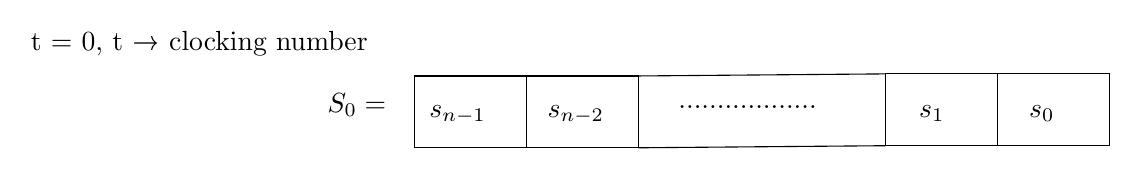
\begin{tikzpicture}[x=0.75pt,y=0.75pt,yscale=-1,xscale=1]
        \draw   (208,107) -- (262,107) -- (262,141.6) -- (208,141.6) -- cycle ; 
        \draw   (262,107) -- (316,107) -- (316,141.6) -- (262,141.6) -- cycle ;
        \draw   (435,106) -- (489,106) -- (489,140.6) -- (435,140.6) -- cycle ;
        \draw    (316,107) -- (435,106) ;
        \draw   (489,106) -- (543,106) -- (543,140.6) -- (489,140.6) -- cycle ;
        \draw    (316,141.6) -- (435,140.6) ;
        
        \draw (214,120) node [anchor=north west][inner sep=0.75pt]   [align=left] {$s_{n-1}$};
        \draw (271,120) node [anchor=north west][inner sep=0.75pt]   [align=left] {$s_{n-2}$};
        \draw (334,120) node [anchor=north west][inner sep=0.75pt]   [align=left] {..................};
        \draw (450,120) node [anchor=north west][inner sep=0.75pt]   [align=left] {$s_1$};
        \draw (503,120) node [anchor=north west][inner sep=0.75pt]   [align=left] {$s_0$};
        \draw (22,84) node [anchor=north west][inner sep=0.75pt]   [align=left] {t = 0, t → clocking number};
        \draw (165,114) node [anchor=north west][inner sep=0.75pt]   [align=left] {$S_0 = $};
    \end{tikzpicture}
\end{center}
At each clocking number, a shift by one bit takes place (either right or left, depends on the design). Here, we will take right shift for understanding.

\begin{center}
    \tikzset{every picture/.style={line width=0.75pt}} 
    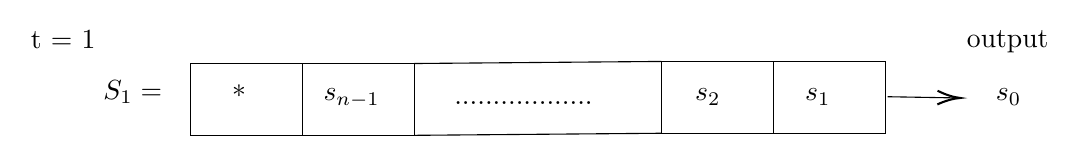
\begin{tikzpicture}[x=0.75pt,y=0.75pt,yscale=-1,xscale=1]
        \draw   (135,197) -- (189,197) -- (189,231.6) -- (135,231.6) -- cycle ;
        \draw   (189,197) -- (243,197) -- (243,231.6) -- (189,231.6) -- cycle ; 
        \draw   (362,196) -- (416,196) -- (416,230.6) -- (362,230.6) -- cycle ;
        \draw    (243,197) -- (362,196) ;
        \draw   (416,196) -- (470,196) -- (470,230.6) -- (416,230.6) -- cycle ;
        \draw    (243,231.6) -- (362,230.6) ;
        \draw    (471,213) -- (504,213.57) ;
        \draw [shift={(506,213.6)}, rotate = 180.98] [color={rgb, 255:red, 0; green, 0; blue, 0 }  ][line width=0.75]    (10.93,-3.29) .. controls (6.95,-1.4) and (3.31,-0.3) .. (0,0) .. controls (3.31,0.3) and (6.95,1.4) .. (10.93,3.29)   ;
        
        \draw (154,206) node [anchor=north west][inner sep=0.75pt]   [align=left] {*};
        \draw (198,208) node [anchor=north west][inner sep=0.75pt]   [align=left] {$s_{n-1}$};
        \draw (261,214) node [anchor=north west][inner sep=0.75pt]   [align=left] {..................};
        \draw (377,208) node [anchor=north west][inner sep=0.75pt]   [align=left] {$s_2$};
        \draw (430,208) node [anchor=north west][inner sep=0.75pt]   [align=left] {$s_1$};
        \draw (57,180) node [anchor=north west][inner sep=0.75pt]   [align=left] {t = 1};
        \draw (92,204) node [anchor=north west][inner sep=0.75pt]   [align=left] {$S_1 =$};
        \draw (508,180) node [anchor=north west][inner sep=0.75pt]   [align=left] {output};
        \draw (522,208) node [anchor=north west][inner sep=0.75pt]   [align=left] {$s_0$};
        
    \end{tikzpicture}
\end{center}

The rightmost bit $s_0$ moves out and is the output (the keystream bit). However, the leftmost bit $s_n$ becomes empty. $s_n$ is known as feedback bit and is calculated as:
\begin{center}
    $s_n = L(s_0, s_1,....., s_{n-1}) = L(S_0)$ 
\end{center}
After one more clocking, the state can be represented as:

\begin{center}
    \tikzset{every picture/.style={line width=0.75pt}} 
    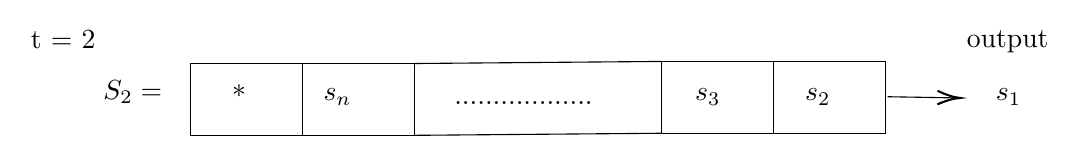
\begin{tikzpicture}[x=0.75pt,y=0.75pt,yscale=-1,xscale=1]
        \draw   (135,197) -- (189,197) -- (189,231.6) -- (135,231.6) -- cycle ;
        \draw   (189,197) -- (243,197) -- (243,231.6) -- (189,231.6) -- cycle ; 
        \draw   (362,196) -- (416,196) -- (416,230.6) -- (362,230.6) -- cycle ;
        \draw    (243,197) -- (362,196) ;
        \draw   (416,196) -- (470,196) -- (470,230.6) -- (416,230.6) -- cycle ;
        \draw    (243,231.6) -- (362,230.6) ;
        \draw    (471,213) -- (504,213.57) ;
        \draw [shift={(506,213.6)}, rotate = 180.98] [color={rgb, 255:red, 0; green, 0; blue, 0 }  ][line width=0.75]    (10.93,-3.29) .. controls (6.95,-1.4) and (3.31,-0.3) .. (0,0) .. controls (3.31,0.3) and (6.95,1.4) .. (10.93,3.29)   ;
        
        \draw (154,206) node [anchor=north west][inner sep=0.75pt]   [align=left] {*};
        \draw (198,208) node [anchor=north west][inner sep=0.75pt]   [align=left] {$s_n$};
        \draw (261,214) node [anchor=north west][inner sep=0.75pt]   [align=left] {..................};
        \draw (377,208) node [anchor=north west][inner sep=0.75pt]   [align=left] {$s_3$};
        \draw (430,208) node [anchor=north west][inner sep=0.75pt]   [align=left] {$s_2$};
        \draw (57,180) node [anchor=north west][inner sep=0.75pt]   [align=left] {t = 2};
        \draw (92,204) node [anchor=north west][inner sep=0.75pt]   [align=left] {$S_2 =$};
        \draw (508,180) node [anchor=north west][inner sep=0.75pt]   [align=left] {output};
        \draw (522,208) node [anchor=north west][inner sep=0.75pt]   [align=left] {$s_1$};
        
    \end{tikzpicture}
\end{center}
Again, the feedback bit $S_{n+1} = L(S_1)$. We will look at the function L in some time. The LFSR with right shift operation can be represented with the following circuit.
\begin{center}
    \tikzset{every picture/.style={line width=0.75pt}} 
    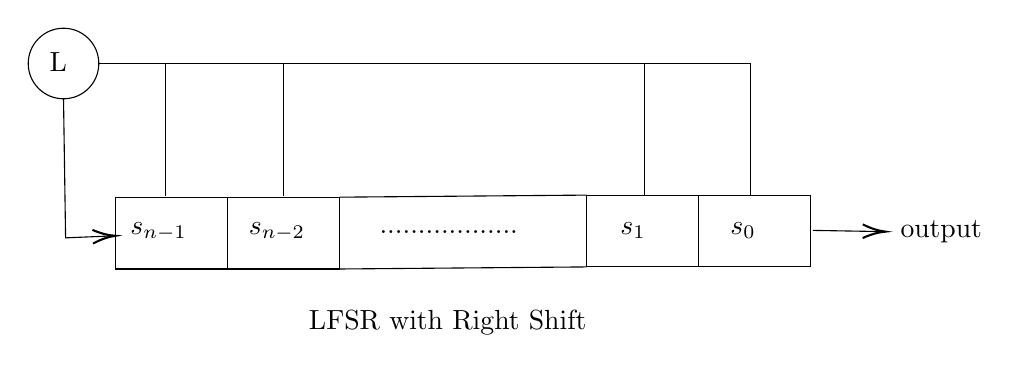
\begin{tikzpicture}[x=0.75pt,y=0.75pt,yscale=-1,xscale=1]
        \draw   (138,147) -- (192,147) -- (192,181.6) -- (138,181.6) -- cycle ;
        \draw   (192,147) -- (246,147) -- (246,181.6) -- (192,181.6) -- cycle ;
        \draw   (365,146) -- (419,146) -- (419,180.6) -- (365,180.6) -- cycle ; 
        \draw    (246,147) -- (365,146) ;
        \draw   (419,146) -- (473,146) -- (473,180.6) -- (419,180.6) -- cycle ;
        \draw    (246,181.6) -- (365,180.6) ; 
        \draw    (474,163) -- (507,163.57) ;
        \draw [shift={(509,163.6)}, rotate = 180.98] [color={rgb, 255:red, 0; green, 0; blue, 0 }  ][line width=0.75]    (10.93,-3.29) .. controls (6.95,-1.4) and (3.31,-0.3) .. (0,0) .. controls (3.31,0.3) and (6.95,1.4) .. (10.93,3.29)   ;
        \draw    (130,82.6) -- (444,82.6) -- (444,146) ;
        \draw   (96,82.6) .. controls (96,73.21) and (103.61,65.6) .. (113,65.6) .. controls (122.39,65.6) and (130,73.21) .. (130,82.6) .. controls (130,91.99) and (122.39,99.6) .. (113,99.6) .. controls (103.61,99.6) and (96,91.99) .. (96,82.6) -- cycle ;
        \draw    (113,99.6) -- (114,166.6) -- (136,165.68) ;
        \draw [shift={(138,165.6)}, rotate = 177.61] [color={rgb, 255:red, 0; green, 0; blue, 0 }  ][line width=0.75]    (10.93,-3.29) .. controls (6.95,-1.4) and (3.31,-0.3) .. (0,0) .. controls (3.31,0.3) and (6.95,1.4) .. (10.93,3.29)   ;
        \draw    (162,82.6) -- (162,146.6) ;
        \draw    (219,82.6) -- (219,146.6) ;
        \draw    (393,82.6) -- (393,146.6) ;
        
        \draw (144,158) node [anchor=north west][inner sep=0.75pt]   [align=left] {$s_{n-1}$};
        \draw (201,158) node [anchor=north west][inner sep=0.75pt]   [align=left] {$s_{n-2}$};
        \draw (264,162) node [anchor=north west][inner sep=0.75pt]   [align=left] {..................};
        \draw (380,158) node [anchor=north west][inner sep=0.75pt]   [align=left] {$s_1$};
        \draw (433,158) node [anchor=north west][inner sep=0.75pt]   [align=left] {$s_0$};
        \draw (515,157) node [anchor=north west][inner sep=0.75pt]   [align=left] {output};
        \draw (105,76) node [anchor=north west][inner sep=0.75pt]   [align=left] {L};
        \draw (230,200) node [anchor=north west][inner sep=0.75pt]   [align=left] {LFSR with Right Shift};
    \end{tikzpicture}
\end{center}

The function L is a linear function on the bits of the previous state.
\begin{center}
    $L: \{0,1\}^n \rightarrow \{0,1\}$\\
    $L(s_0, s_1,....., s_{n-1}) = s_n$
\end{center}
A linear function can be represented as:
\begin{center}
    $L_a = a_0\cdot s_0 \oplus a_1 \cdot s_1 \oplus ..... \oplus a_{n-1} \cdot s_{n-1}$ where $a_i \in \{0, 1\}$
\end{center}

Suppose, an arbitrary function L be defined as:
\begin{center}
    $L = a_0\cdot s_0 \oplus a_1 \cdot s_1 \oplus ..... \oplus a_{n-1} \cdot s_{n-1} \oplus a_n$ where $a_i \in \{0, 1\}$
\end{center}
In this function, if $a_n = 0$ then $L = L_a$, a linear function. Otherwise, if $a_n = 1$ the $L \neq L_a$. In fact, such a function is known as Affine function.

A function can be proved to be linear using the following property.
\begin{center}
    $L(X) \oplus L(Y) = L(X \oplus Y)$\\
    $\implies L(X) \oplus L(Y) \oplus L(X \oplus Y) = 0$
\end{center}
\textbf{Example:} Find if the following functions are linear or not. Solve it considering 2-bit inputs.
\begin{enumerate}
    \item $L_1(x, y) = x \oplus y$
    \item $L_2(x, y) = 1 \oplus x \oplus y$

\end{enumerate}
\textbf{Solution:} 
\begin{enumerate}
    \item Let's compute $L_1(x) \oplus L_1(y) \oplus L_1(x \oplus y)$
    \begin{center}
        $L_1(x) \oplus L_1(y) \oplus L_1(x \oplus y) = (x_1 \oplus x_2) \oplus (y_1 \oplus y_2) \oplus ((x_1 \oplus y_1) \oplus (x_2 \oplus y_2))$\\
        \vspace{1mm}
        $L_1(x) \oplus L_1(y) \oplus L_1(x \oplus y) = 0$
    \end{center}
    Therefore, $L_1$ is a linear function.
    \item $L_2(x) \oplus L_2(y) \oplus L_2(x \oplus y) = (1 \oplus x_1 \oplus x_2) \oplus (1 \oplus y_1 \oplus y_2) \oplus (1 \oplus (x_1 \oplus y_1) \oplus (x_2 \oplus y_2))$
    \begin{center}
        $L_2(x) \oplus L_2(y) \oplus L_2(x \oplus y) = 1 $
    \end{center}
    Therefore, $L_2$ is not a linear function.
\end{enumerate}

LFSR has a linear function, whose output depends on previous state, therefore it provides feedback. There is shift operation on the bits stored in register. Hence, the name is Linear Feedback Shift Register. \\
Now, let us see an example of a 3-bit LFSR.

\begin{center}
    \tikzset{every picture/.style={line width=0.75pt}}
    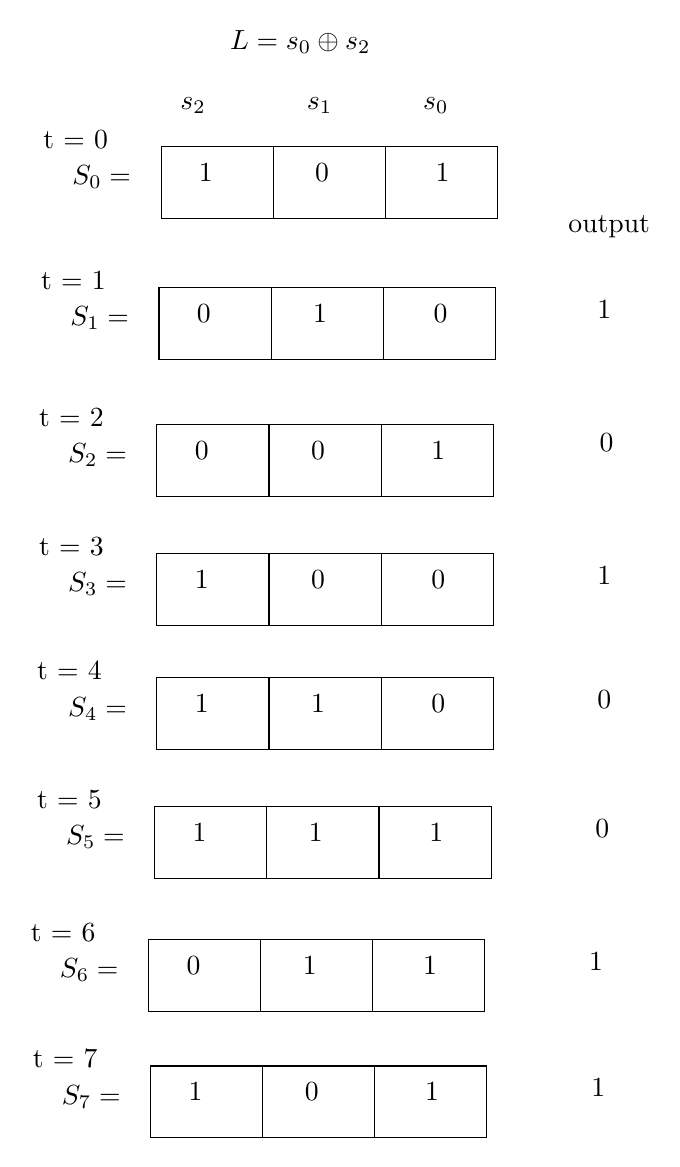
\begin{tikzpicture}[x=0.75pt,y=0.75pt,yscale=-1,xscale=1]
        
        \draw   (230,277) -- (284,277) -- (284,311.6) -- (230,311.6) -- cycle ;
        \draw   (284,277) -- (338,277) -- (338,311.6) -- (284,311.6) -- cycle ;
        \draw   (338,277) -- (392,277) -- (392,311.6) -- (338,311.6) -- cycle ;
        \draw   (229,345) -- (283,345) -- (283,379.6) -- (229,379.6) -- cycle ;
        \draw   (283,345) -- (337,345) -- (337,379.6) -- (283,379.6) -- cycle ;
        \draw   (337,345) -- (391,345) -- (391,379.6) -- (337,379.6) -- cycle ;
        \draw   (228,411) -- (282,411) -- (282,445.6) -- (228,445.6) -- cycle ;
        \draw   (282,411) -- (336,411) -- (336,445.6) -- (282,445.6) -- cycle ;
        \draw   (336,411) -- (390,411) -- (390,445.6) -- (336,445.6) -- cycle ;
        \draw   (228,473) -- (282,473) -- (282,507.6) -- (228,507.6) -- cycle ;
        \draw   (282,473) -- (336,473) -- (336,507.6) -- (282,507.6) -- cycle ;
        \draw   (336,473) -- (390,473) -- (390,507.6) -- (336,507.6) -- cycle ;
        \draw   (228,533) -- (282,533) -- (282,567.6) -- (228,567.6) -- cycle ;
        \draw   (282,533) -- (336,533) -- (336,567.6) -- (282,567.6) -- cycle ;
        \draw   (336,533) -- (390,533) -- (390,567.6) -- (336,567.6) -- cycle ;
        \draw   (227,595) -- (281,595) -- (281,629.6) -- (227,629.6) -- cycle ;
        \draw   (281,595) -- (335,595) -- (335,629.6) -- (281,629.6) -- cycle ;
        \draw   (335,595) -- (389,595) -- (389,629.6) -- (335,629.6) -- cycle ;
        \draw   (224,659) -- (278,659) -- (278,693.6) -- (224,693.6) -- cycle ;
        \draw   (278,659) -- (332,659) -- (332,693.6) -- (278,693.6) -- cycle ;
        \draw   (332,659) -- (386,659) -- (386,693.6) -- (332,693.6) -- cycle ;
        \draw   (225,720) -- (279,720) -- (279,754.6) -- (225,754.6) -- cycle ;
        \draw   (279,720) -- (333,720) -- (333,754.6) -- (279,754.6) -- cycle ;
        \draw   (333,720) -- (387,720) -- (387,754.6) -- (333,754.6) -- cycle ;
        
        \draw (303,284) node [anchor=north west][inner sep=0.75pt]   [align=left] {0};
        \draw (262,220) node [anchor=north west][inner sep=0.75pt]   [align=left] {$L = s_0 \oplus s_2$};
        \draw (238,252) node [anchor=north west][inner sep=0.75pt]   [align=left] {$s_2$};
        \draw (299,252) node [anchor=north west][inner sep=0.75pt]   [align=left] {$s_1$};
        \draw (355,252) node [anchor=north west][inner sep=0.75pt]   [align=left] {$s_0$};
        \draw (172,268) node [anchor=north west][inner sep=0.75pt]   [align=left] {t = 0};
        \draw (186,285) node [anchor=north west][inner sep=0.75pt]   [align=left] {$S_0 = $};
        \draw (425,309) node [anchor=north west][inner sep=0.75pt]   [align=left] {output};
        \draw (247,284) node [anchor=north west][inner sep=0.75pt]   [align=left] {1};
        \draw (361,284) node [anchor=north west][inner sep=0.75pt]   [align=left] {1};
        \draw (302,352) node [anchor=north west][inner sep=0.75pt]   [align=left] {1};
        \draw (171,336) node [anchor=north west][inner sep=0.75pt]   [align=left] {t = 1};
        \draw (185,353) node [anchor=north west][inner sep=0.75pt]   [align=left] {$S_1 = $};
        \draw (246,352) node [anchor=north west][inner sep=0.75pt]   [align=left] {0};
        \draw (360,352) node [anchor=north west][inner sep=0.75pt]   [align=left] {0};
        \draw (301,418) node [anchor=north west][inner sep=0.75pt]   [align=left] {0};
        \draw (170,402) node [anchor=north west][inner sep=0.75pt]   [align=left] {t = 2};
        \draw (184,419) node [anchor=north west][inner sep=0.75pt]   [align=left] {$S_2 = $};
        \draw (245,418) node [anchor=north west][inner sep=0.75pt]   [align=left] {0};
        \draw (359,418) node [anchor=north west][inner sep=0.75pt]   [align=left] {1};
        \draw (301,480) node [anchor=north west][inner sep=0.75pt]   [align=left] {0};
        \draw (170,464) node [anchor=north west][inner sep=0.75pt]   [align=left] {t = 3};
        \draw (184,481) node [anchor=north west][inner sep=0.75pt]   [align=left] {$S_3 = $};
        \draw (245,480) node [anchor=north west][inner sep=0.75pt]   [align=left] {1};
        \draw (359,480) node [anchor=north west][inner sep=0.75pt]   [align=left] {0};
        \draw (439,350) node [anchor=north west][inner sep=0.75pt]   [align=left] {1};
        \draw (440,414) node [anchor=north west][inner sep=0.75pt]   [align=left] {0};
        \draw (439,478) node [anchor=north west][inner sep=0.75pt]   [align=left] {1};
        \draw (301,540) node [anchor=north west][inner sep=0.75pt]   [align=left] {1};
        \draw (169,524) node [anchor=north west][inner sep=0.75pt]   [align=left] {t = 4};
        \draw (184,541) node [anchor=north west][inner sep=0.75pt]   [align=left] {$S_4 = $};
        \draw (245,540) node [anchor=north west][inner sep=0.75pt]   [align=left] {1};
        \draw (359,540) node [anchor=north west][inner sep=0.75pt]   [align=left] {0};
        \draw (439,538) node [anchor=north west][inner sep=0.75pt]   [align=left] {0};
        \draw (300,602) node [anchor=north west][inner sep=0.75pt]   [align=left] {1};
        \draw (169,586) node [anchor=north west][inner sep=0.75pt]   [align=left] {t = 5};
        \draw (183,603) node [anchor=north west][inner sep=0.75pt]   [align=left] {$S_5 = $};
        \draw (244,602) node [anchor=north west][inner sep=0.75pt]   [align=left] {1};
        \draw (358,602) node [anchor=north west][inner sep=0.75pt]   [align=left] {1};
        \draw (438,600) node [anchor=north west][inner sep=0.75pt]   [align=left] {0};
        \draw (297,666) node [anchor=north west][inner sep=0.75pt]   [align=left] {1};
        \draw (166,650) node [anchor=north west][inner sep=0.75pt]   [align=left] {t = 6};
        \draw (180,667) node [anchor=north west][inner sep=0.75pt]   [align=left] {$S_6 = $};
        \draw (241,666) node [anchor=north west][inner sep=0.75pt]   [align=left] {0};
        \draw (355,666) node [anchor=north west][inner sep=0.75pt]   [align=left] {1};
        \draw (435,664) node [anchor=north west][inner sep=0.75pt]   [align=left] {1};
        \draw (298,727) node [anchor=north west][inner sep=0.75pt]   [align=left] {0};
        \draw (167,711) node [anchor=north west][inner sep=0.75pt]   [align=left] {t = 7};
        \draw (181,728) node [anchor=north west][inner sep=0.75pt]   [align=left] {$S_7 = $};
        \draw (242,727) node [anchor=north west][inner sep=0.75pt]   [align=left] {1};
        \draw (356,727) node [anchor=north west][inner sep=0.75pt]   [align=left] {1};
        \draw (436,725) node [anchor=north west][inner sep=0.75pt]   [align=left] {1};        
    \end{tikzpicture}
\end{center}

The L function for this LFSR is $L = s_0 \oplus s_2$.\\
In any LFSR, if you have reached the initial state again, the the output bits will be repeated. In the above example it can be seen that from start state t = 0 to the state t = 7, all the non-zero states are obtained.\\
The output bits in the above example are repeated after $t = 2^3 - 1$ states because at t = 7, the initial state is reached. Hence, maximum output length that can be achieved in this LFSR without repetition is 7.
Hence, using LFSR, only $2^n - 1$ maximum number of non-zero states can be generated.\\
Also, if we take the 0 state i.e. all bits in the register are 0, it will remain in the zero state forever. Hence, in any LFSR, if input state is 0, then it will remain zero. Hence, LFSR has a fixed point (0-state).\\

Let us look at another example of a 3-bit LFSR with a different L function. This time the L function is $L = s_0$.

\begin{center}   
    \tikzset{every picture/.style={line width=0.75pt}}
    \begin{tikzpicture}[x=0.75pt,y=0.75pt,yscale=-1,xscale=1]
        \draw   (230,277) -- (284,277) -- (284,311.6) -- (230,311.6) -- cycle ;
        \draw   (284,277) -- (338,277) -- (338,311.6) -- (284,311.6) -- cycle ; 
        \draw   (338,277) -- (392,277) -- (392,311.6) -- (338,311.6) -- cycle ; 
        \draw   (229,345) -- (283,345) -- (283,379.6) -- (229,379.6) -- cycle ;
        \draw   (283,345) -- (337,345) -- (337,379.6) -- (283,379.6) -- cycle ;
        \draw   (337,345) -- (391,345) -- (391,379.6) -- (337,379.6) -- cycle ;
        \draw   (228,411) -- (282,411) -- (282,445.6) -- (228,445.6) -- cycle ;
        \draw   (282,411) -- (336,411) -- (336,445.6) -- (282,445.6) -- cycle ;
        \draw   (336,411) -- (390,411) -- (390,445.6) -- (336,445.6) -- cycle ;
        \draw   (228,473) -- (282,473) -- (282,507.6) -- (228,507.6) -- cycle ;
        \draw   (282,473) -- (336,473) -- (336,507.6) -- (282,507.6) -- cycle ;
        \draw   (336,473) -- (390,473) -- (390,507.6) -- (336,507.6) -- cycle ;
        
        
        \draw (303,284) node [anchor=north west][inner sep=0.75pt]   [align=left] {0};
        \draw (290,220) node [anchor=north west][inner sep=0.75pt]   [align=left] {$L = s0$};
        \draw (238,252) node [anchor=north west][inner sep=0.75pt]   [align=left] {$s_2$};
        \draw (299,252) node [anchor=north west][inner sep=0.75pt]   [align=left] {$s_1$};
        \draw (355,252) node [anchor=north west][inner sep=0.75pt]   [align=left] {$s_0$};
        \draw (172,268) node [anchor=north west][inner sep=0.75pt]   [align=left] {t = 0};
        \draw (186,285) node [anchor=north west][inner sep=0.75pt]   [align=left] {$S_0 = $};
        \draw (425,309) node [anchor=north west][inner sep=0.75pt]   [align=left] {output};
        \draw (247,284) node [anchor=north west][inner sep=0.75pt]   [align=left] {1};
        \draw (361,284) node [anchor=north west][inner sep=0.75pt]   [align=left] {1};
        \draw (302,352) node [anchor=north west][inner sep=0.75pt]   [align=left] {1};
        \draw (171,336) node [anchor=north west][inner sep=0.75pt]   [align=left] {t = 1};
        \draw (185,353) node [anchor=north west][inner sep=0.75pt]   [align=left] {$S_1 = $};
        \draw (246,352) node [anchor=north west][inner sep=0.75pt]   [align=left] {1};
        \draw (360,352) node [anchor=north west][inner sep=0.75pt]   [align=left] {0};
        \draw (301,418) node [anchor=north west][inner sep=0.75pt]   [align=left] {1};
        \draw (170,402) node [anchor=north west][inner sep=0.75pt]   [align=left] {t = 2};
        \draw (184,419) node [anchor=north west][inner sep=0.75pt]   [align=left] {$S_2 = $};
        \draw (245,418) node [anchor=north west][inner sep=0.75pt]   [align=left] {0};
        \draw (359,418) node [anchor=north west][inner sep=0.75pt]   [align=left] {1};
        \draw (301,480) node [anchor=north west][inner sep=0.75pt]   [align=left] {0};
        \draw (170,464) node [anchor=north west][inner sep=0.75pt]   [align=left] {t = 3};
        \draw (184,481) node [anchor=north west][inner sep=0.75pt]   [align=left] {$S_3 = $};
        \draw (245,480) node [anchor=north west][inner sep=0.75pt]   [align=left] {1};
        \draw (359,480) node [anchor=north west][inner sep=0.75pt]   [align=left] {1};
        \draw (439,350) node [anchor=north west][inner sep=0.75pt]   [align=left] {1};
        \draw (440,414) node [anchor=north west][inner sep=0.75pt]   [align=left] {0};
        \draw (439,478) node [anchor=north west][inner sep=0.75pt]   [align=left] {1};        
    \end{tikzpicture}
\end{center}
Here, we can see the initial state is reached again only at t = 3. For LFSR, the linear functionis very important in deciding the period after which the bits will repeat.

\subsubsection{Period of an LFSR} 
Consider $S_0$ to be a non-zero state. $S_0$ is repeated after $m$ clocking of LFSR, then $m$ will be the period of LFSR. An LFSR with n-bits can have a maximum period of $2^n - 1$.\\


If there is an LFSR where different non-zero states are repeating at certain different number of clocking. Let us say $x_1$ number of states repeat after $P_1$ clocking, $x_2$ number of states repeat after $P_2$ clocking and so on $x_n$ number of states repeat after $P_N$ clocking. Here, every non-zero state is present in at least and only one $x_i$. Therefore, if we take any non-zero state, then it will repeat after certain number of clocking which will belong to the set $\{P_1, P_2,...., P_N\}$. Therefore, the period of LFSR will be:
\begin{center}
    Period of LFSR = $LCM(P_1, P_2,...., P_N)$
\end{center}
Consider an n-bit LFSR,
\begin{center}
    \tikzset{every picture/.style={line width=0.75pt}} 
    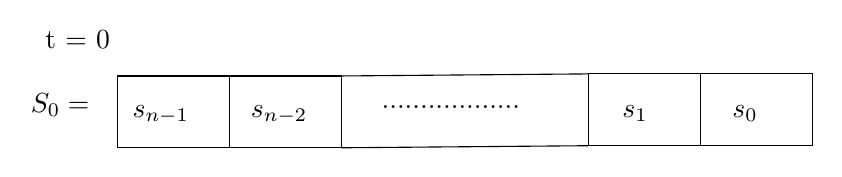
\begin{tikzpicture}[x=0.75pt,y=0.75pt,yscale=-1,xscale=1]
        \draw   (208,107) -- (262,107) -- (262,141.6) -- (208,141.6) -- cycle ; 
        \draw   (262,107) -- (316,107) -- (316,141.6) -- (262,141.6) -- cycle ;
        \draw   (435,106) -- (489,106) -- (489,140.6) -- (435,140.6) -- cycle ;
        \draw    (316,107) -- (435,106) ;
        \draw   (489,106) -- (543,106) -- (543,140.6) -- (489,140.6) -- cycle ;
        \draw    (316,141.6) -- (435,140.6) ;
        
        \draw (214,120) node [anchor=north west][inner sep=0.75pt]   [align=left] {$s_{n-1}$};
        \draw (271,120) node [anchor=north west][inner sep=0.75pt]   [align=left] {$s_{n-2}$};
        \draw (334,120) node [anchor=north west][inner sep=0.75pt]   [align=left] {..................};
        \draw (450,120) node [anchor=north west][inner sep=0.75pt]   [align=left] {$s_1$};
        \draw (503,120) node [anchor=north west][inner sep=0.75pt]   [align=left] {$s_0$};
        \draw (172,84) node [anchor=north west][inner sep=0.75pt]   [align=left] {t = 0};
        \draw (165,114) node [anchor=north west][inner sep=0.75pt]   [align=left] {$S_0 = $};
    \end{tikzpicture}
\end{center}
We know that after clocking, $s_n$ will be,
\begin{center}
    $s_n = L(s_0,s_1,...., s_{n-1})$\\
    $s_n = c_1\cdot s_{n-1} \oplus c_2 \cdot s_{n-2} \oplus ..... \oplus c_n \cdot s_0$ where $c_i \in \{0, 1\}$
\end{center}
This is known as Algebraic Normal Form of writing $s_n$. Therefore, we can see that to implement LFSR in hardware, we only need AND and XOR gates. The circuit for LFSR is given below. The value of $s_i$ will be xored or not depends on the value of $c_{n-i}$.

\begin{center}
    \tikzset{every picture/.style={line width=0.75pt}} 
    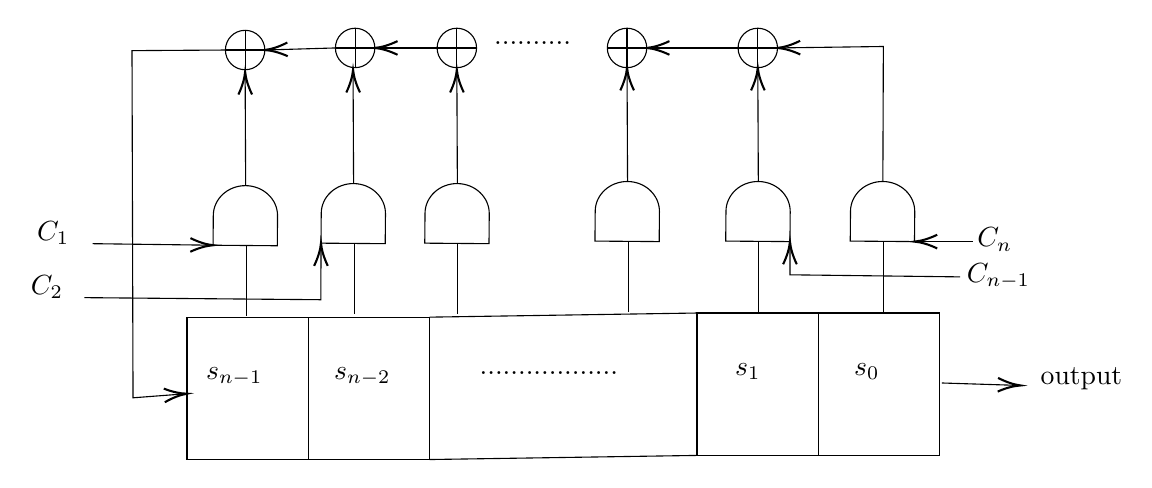
\begin{tikzpicture}[x=0.75pt,y=0.75pt,yscale=-1,xscale=1]
        \draw   (110.47,177.2) -- (168.93,177.2) -- (168.93,245.8) -- (110.47,245.8) -- cycle ;
        \draw   (168.93,177.2) -- (227.39,177.2) -- (227.39,245.8) -- (168.93,245.8) -- cycle ;
        \draw   (356.22,175.21) -- (414.68,175.21) -- (414.68,243.82) -- (356.22,243.82) -- cycle ; 
        \draw    (227.39,177.2) -- (356.22,175.21) ;
        \draw   (414.68,175.21) -- (473.14,175.21) -- (473.14,243.82) -- (414.68,243.82) -- cycle ;
        \draw    (227.39,245.8) -- (356.22,243.82) ;
        \draw    (474.22,208.92) -- (510.11,210.05) ;
        \draw [shift={(512.11,210.11)}, rotate = 181.8] [color={rgb, 255:red, 0; green, 0; blue, 0 }  ][line width=0.75]    (10.93,-3.29) .. controls (6.95,-1.4) and (3.31,-0.3) .. (0,0) .. controls (3.31,0.3) and (6.95,1.4) .. (10.93,3.29)   ;
        \draw    (129,48.5) -- (84,48.8) -- (84.49,216.06) -- (108.47,214.23) ;
        \draw [shift={(110.47,214.08)}, rotate = 175.64] [color={rgb, 255:red, 0; green, 0; blue, 0 }  ][line width=0.75]    (10.93,-3.29) .. controls (6.95,-1.4) and (3.31,-0.3) .. (0,0) .. controls (3.31,0.3) and (6.95,1.4) .. (10.93,3.29)   ;
        \draw   (370.05,140.55) -- (370.17,126.13) .. controls (370.24,118.17) and (377.22,111.77) .. (385.76,111.84) .. controls (394.31,111.91) and (401.18,118.42) .. (401.12,126.38) -- (401,140.8) -- cycle ;
        \draw    (386,140.8) -- (386,174.8) ; 
        \draw   (129,48.5) .. controls (129,43.25) and (133.25,39) .. (138.5,39) .. controls (143.75,39) and (148,43.25) .. (148,48.5) .. controls (148,53.75) and (143.75,58) .. (138.5,58) .. controls (133.25,58) and (129,53.75) .. (129,48.5) -- cycle ; \draw   (129,48.5) -- (148,48.5) ; \draw   (138.5,39) -- (138.5,58) ;
        \draw   (182,47.5) .. controls (182,42.25) and (186.25,38) .. (191.5,38) .. controls (196.75,38) and (201,42.25) .. (201,47.5) .. controls (201,52.75) and (196.75,57) .. (191.5,57) .. controls (186.25,57) and (182,52.75) .. (182,47.5) -- cycle ; \draw   (182,47.5) -- (201,47.5) ; \draw   (191.5,38) -- (191.5,57) ;
        \draw   (231,47.5) .. controls (231,42.25) and (235.25,38) .. (240.5,38) .. controls (245.75,38) and (250,42.25) .. (250,47.5) .. controls (250,52.75) and (245.75,57) .. (240.5,57) .. controls (235.25,57) and (231,52.75) .. (231,47.5) -- cycle ; \draw   (231,47.5) -- (250,47.5) ; \draw   (240.5,38) -- (240.5,57) ;
        \draw   (313,47.5) .. controls (313,42.25) and (317.25,38) .. (322.5,38) .. controls (327.75,38) and (332,42.25) .. (332,47.5) .. controls (332,52.75) and (327.75,57) .. (322.5,57) .. controls (317.25,57) and (313,52.75) .. (313,47.5) -- cycle ; \draw   (313,47.5) -- (332,47.5) ; \draw   (322.5,38) -- (322.5,57) ;
        \draw   (376,47.5) .. controls (376,42.25) and (380.25,38) .. (385.5,38) .. controls (390.75,38) and (395,42.25) .. (395,47.5) .. controls (395,52.75) and (390.75,57) .. (385.5,57) .. controls (380.25,57) and (376,52.75) .. (376,47.5) -- cycle ; \draw   (376,47.5) -- (395,47.5) ; \draw   (385.5,38) -- (385.5,57) ;
        \draw    (376,47.5) -- (334,47.5) ;
        \draw [shift={(332,47.5)}, rotate = 360] [color={rgb, 255:red, 0; green, 0; blue, 0 }  ][line width=0.75]    (10.93,-3.29) .. controls (6.95,-1.4) and (3.31,-0.3) .. (0,0) .. controls (3.31,0.3) and (6.95,1.4) .. (10.93,3.29)   ;
        \draw    (231,47.5) -- (203,47.5) ;
        \draw [shift={(201,47.5)}, rotate = 360] [color={rgb, 255:red, 0; green, 0; blue, 0 }  ][line width=0.75]    (10.93,-3.29) .. controls (6.95,-1.4) and (3.31,-0.3) .. (0,0) .. controls (3.31,0.3) and (6.95,1.4) .. (10.93,3.29)   ;
        \draw    (182,47.5) -- (150,48.44) ;
        \draw [shift={(148,48.5)}, rotate = 358.32] [color={rgb, 255:red, 0; green, 0; blue, 0 }  ][line width=0.75]    (10.93,-3.29) .. controls (6.95,-1.4) and (3.31,-0.3) .. (0,0) .. controls (3.31,0.3) and (6.95,1.4) .. (10.93,3.29)   ;
        \draw    (385.76,111.84) -- (385.51,59) ;
        \draw [shift={(385.5,57)}, rotate = 89.73] [color={rgb, 255:red, 0; green, 0; blue, 0 }  ][line width=0.75]    (10.93,-3.29) .. controls (6.95,-1.4) and (3.31,-0.3) .. (0,0) .. controls (3.31,0.3) and (6.95,1.4) .. (10.93,3.29)   ;
        \draw   (307.05,140.55) -- (307.17,126.13) .. controls (307.24,118.17) and (314.22,111.77) .. (322.76,111.84) .. controls (331.31,111.91) and (338.18,118.42) .. (338.12,126.38) -- (338,140.8) -- cycle ;
        \draw    (323,140.8) -- (323,174.8) ;
        \draw    (322.76,111.84) -- (322.51,59) ;
        \draw [shift={(322.5,57)}, rotate = 89.73] [color={rgb, 255:red, 0; green, 0; blue, 0 }  ][line width=0.75]    (10.93,-3.29) .. controls (6.95,-1.4) and (3.31,-0.3) .. (0,0) .. controls (3.31,0.3) and (6.95,1.4) .. (10.93,3.29)   ;
        \draw   (225.05,141.55) -- (225.17,127.13) .. controls (225.24,119.17) and (232.22,112.77) .. (240.76,112.84) .. controls (249.31,112.91) and (256.18,119.42) .. (256.12,127.38) -- (256,141.8) -- cycle ;
        \draw    (241,141.8) -- (241,175.8) ; 
        \draw    (240.76,112.84) -- (240.51,60) ;
        \draw [shift={(240.5,58)}, rotate = 89.73] [color={rgb, 255:red, 0; green, 0; blue, 0 }  ][line width=0.75]    (10.93,-3.29) .. controls (6.95,-1.4) and (3.31,-0.3) .. (0,0) .. controls (3.31,0.3) and (6.95,1.4) .. (10.93,3.29)   ;
        \draw   (175.05,141.55) -- (175.17,127.13) .. controls (175.24,119.17) and (182.22,112.77) .. (190.76,112.84) .. controls (199.31,112.91) and (206.18,119.42) .. (206.12,127.38) -- (206,141.8) -- cycle ;
        \draw    (191,141.8) -- (191,175.8) ; 
        \draw    (190.76,112.84) -- (190.51,60) ;
        \draw [shift={(190.5,58)}, rotate = 89.73] [color={rgb, 255:red, 0; green, 0; blue, 0 }  ][line width=0.75]    (10.93,-3.29) .. controls (6.95,-1.4) and (3.31,-0.3) .. (0,0) .. controls (3.31,0.3) and (6.95,1.4) .. (10.93,3.29)   ; 
        \draw   (123.05,142.55) -- (123.17,128.13) .. controls (123.24,120.17) and (130.22,113.77) .. (138.76,113.84) .. controls (147.31,113.91) and (154.18,120.42) .. (154.12,128.38) -- (154,142.8) -- cycle ;
        \draw    (139,142.8) -- (139,176.8) ;
        \draw    (138.76,113.84) -- (138.51,61) ;
        \draw [shift={(138.5,59)}, rotate = 89.73] [color={rgb, 255:red, 0; green, 0; blue, 0 }  ][line width=0.75]    (10.93,-3.29) .. controls (6.95,-1.4) and (3.31,-0.3) .. (0,0) .. controls (3.31,0.3) and (6.95,1.4) .. (10.93,3.29)   ;
        \draw   (430.05,140.55) -- (430.17,126.13) .. controls (430.24,118.17) and (437.22,111.77) .. (445.76,111.84) .. controls (454.31,111.91) and (461.18,118.42) .. (461.12,126.38) -- (461,140.8) -- cycle ;
        \draw    (446,140.8) -- (446,174.8) ;
        \draw    (445.76,111.84) -- (446,46.8) -- (397,47.47) ;
        \draw [shift={(395,47.5)}, rotate = 359.21] [color={rgb, 255:red, 0; green, 0; blue, 0 }  ][line width=0.75]    (10.93,-3.29) .. controls (6.95,-1.4) and (3.31,-0.3) .. (0,0) .. controls (3.31,0.3) and (6.95,1.4) .. (10.93,3.29)   ;
        \draw    (489,140.8) -- (463,140.8) ;
        \draw [shift={(461,140.8)}, rotate = 360] [color={rgb, 255:red, 0; green, 0; blue, 0 }  ][line width=0.75]    (10.93,-3.29) .. controls (6.95,-1.4) and (3.31,-0.3) .. (0,0) .. controls (3.31,0.3) and (6.95,1.4) .. (10.93,3.29)   ;
        \draw    (483,157.8) -- (401,156.8) -- (401,142.8) ;
        \draw [shift={(401,140.8)}, rotate = 90] [color={rgb, 255:red, 0; green, 0; blue, 0 }  ][line width=0.75]    (10.93,-3.29) .. controls (6.95,-1.4) and (3.31,-0.3) .. (0,0) .. controls (3.31,0.3) and (6.95,1.4) .. (10.93,3.29)   ;
        \draw    (61,167.8) -- (175,168.8) -- (175.05,143.55) ;
        \draw [shift={(175.05,141.55)}, rotate = 90.11] [color={rgb, 255:red, 0; green, 0; blue, 0 }  ][line width=0.75]    (10.93,-3.29) .. controls (6.95,-1.4) and (3.31,-0.3) .. (0,0) .. controls (3.31,0.3) and (6.95,1.4) .. (10.93,3.29)   ;
        \draw    (65,141.8) -- (121.05,142.52) ;
        \draw [shift={(123.05,142.55)}, rotate = 180.74] [color={rgb, 255:red, 0; green, 0; blue, 0 }  ][line width=0.75]    (10.93,-3.29) .. controls (6.95,-1.4) and (3.31,-0.3) .. (0,0) .. controls (3.31,0.3) and (6.95,1.4) .. (10.93,3.29)   ;
        
        \draw (118.41,200.39) node [anchor=north west][inner sep=0.75pt]   [align=left] {$s_{n-1}$};
        \draw (180.12,200.39) node [anchor=north west][inner sep=0.75pt]   [align=left] {$s_{n-2}$};
        \draw (250.22,202.38) node [anchor=north west][inner sep=0.75pt]   [align=left] {..................};
        \draw (373.32,198.41) node [anchor=north west][inner sep=0.75pt]   [align=left] {$s_1$};
        \draw (430.7,198.41) node [anchor=north west][inner sep=0.75pt]   [align=left] {$s_0$};
        \draw (520.55,200.39) node [anchor=north west][inner sep=0.75pt]   [align=left] {output};
        \draw (257.22,43.38) node [anchor=north west][inner sep=0.75pt]   [align=left] {..........};
        \draw (490,133) node [anchor=north west][inner sep=0.75pt]   [align=left] {$C_n$};
        \draw (485,150) node [anchor=north west][inner sep=0.75pt]   [align=left] {$C_{n-1}$};
        \draw (34,156) node [anchor=north west][inner sep=0.75pt]   [align=left] {$C_2$};
        \draw (37,130) node [anchor=north west][inner sep=0.75pt]   [align=left] {$C_1$};        
    \end{tikzpicture}
\end{center}



Corresponding to every LFSR, we have a Linear Feedback Function (L). Corresponding to LFF, we can construct a polynomial $f(x)$.
\begin{center}
    $L = c_1\cdot s_{n-1} \oplus c_2 \cdot s_{n-2} \oplus ..... \oplus c_n \cdot s_0$\\
    $f(x) = 1 + c_1 \cdot x + c_2 \cdot x^2 + ..... + c_n \cdot x^n$
\end{center}
The polynomial $f(x)$ is known as connection polynomial of LFSR. If anyone of the linear feedback function or the connection poylnomial is known, the other can be easily constructed. Since, $c_i \in \{0, 1\}$ for $1 \leq i \leq n$, therefore, $f(x) \in F_2[x]$. Therefore, 
\begin{center}
    n-bit LFSR $\iff$ Linear Feedback Function $\iff$ one polynomial in $F_2[x]$ of degree $\leq n$
\end{center}
We know that is $S_0$ repeats after $2^n - 1$ clocking, then it is a full period LFSR. Now, consider a connection polynomial of degree n in $F_2[x]$.

\begin{enumerate}
    \item If the connection polynomial is primitive polynomial, then the LFSR will have full period.\\
    \newline
    If we recall, during AES we studied that if $G(x)$ is a primitive polynomial, then $(F_2[x]/\langle G(x)\rangle, +, *)$ is a field where $F_2[x]/\langle G(x)\rangle$ contains all polynomials with degree less than degree of G(x). Similarly, here we have a n degree connection polynomial. If it is primitive, then we can construct all polynomials of degree less than n. That is, we can construct $2^n - 1$ polynomials. Therefore, we can generate all the possible non-zero states of LFSR.

    \item If connecting polynomial is irreducible (and not primitive), $F_2[x]/\langle G(x)\rangle$, then the period of LFSR will divide $2^n-1$.

    \item If connecting polynomial is reducible, then different states will have different cycle length (different period).
\end{enumerate}


\subsection*{Security of Linear Feedback Shift Register (LFSR)}

In the context of Linear Feedback Shift Registers (LFSRs), the confidential key is commonly stored within the register's memory. The register comprises \( n \) bits, denoted as \( K \), where \( K = K_0K_1 \ldots K_{n-1} \). Typically, the secret key or other essential parameters are stored in this register, and from it, output bits \( x_i \) are generated, serving as keystream bits \( Z_i \). These keystream bits are pivotal in encryption processes, where the relationship \( m_i \oplus Z_i = C_i \) denotes the ciphertext bits. Each clock cycle of the LFSR yields one output bit and involves a feedback mechanism. In scenarios like the Known Plaintext Attack Model, where specific plaintext and corresponding ciphertext bits are disclosed, the goal is to ascertain the secret key \( K \).
 Given \(m_i\) and \(c_i\), we can calculate \(Z_i\) as:

\[ Z_i = m_i \oplus C_i \]

Thus, we have \(Z_i\) corresponding to the known \(m_i\) and \(C_i\). Since the first output bit according to the LFSR is \(K_0\), the second output bit is \(K_1\), and so on, if we know the first \(n\) bits of the message and corresponding ciphertext, we can obtain the entire secret key.


\subsubsection{LFSR with Non-Linear Filter Function}
Here, we will consider an l-bit boolean function $f$ which takes l-bits as input and produces one bit as output. We will take l-bits out of the n-bits of the state of LFSR as input to f and use the output of $f$ as $Z_i \in \{0, 1\}$. The function $f$ here is a non-linear function.
\begin{center}
    \tikzset{every picture/.style={line width=0.75pt}}        
    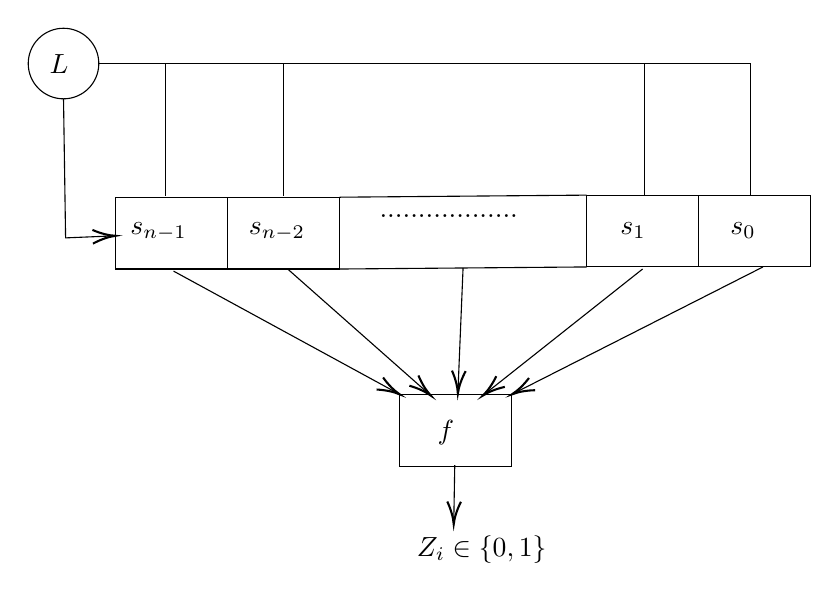
\begin{tikzpicture}[x=0.75pt,y=0.75pt,yscale=-1,xscale=1]
        \draw   (138,1067.4) -- (192,1067.4) -- (192,1102) -- (138,1102) -- cycle ;
        \draw   (192,1067.4) -- (246,1067.4) -- (246,1102) -- (192,1102) -- cycle ;
        \draw   (365,1066.4) -- (419,1066.4) -- (419,1101) -- (365,1101) -- cycle ;
        \draw    (246,1067.4) -- (365,1066.4) ;
        \draw   (419,1066.4) -- (473,1066.4) -- (473,1101) -- (419,1101) -- cycle ; 
        \draw    (246,1102) -- (365,1101) ;
        \draw    (166,1103) -- (273.24,1161.44) ;
        \draw [shift={(275,1162.4)}, rotate = 208.59] [color={rgb, 255:red, 0; green, 0; blue, 0 }  ][line width=0.75]    (10.93,-3.29) .. controls (6.95,-1.4) and (3.31,-0.3) .. (0,0) .. controls (3.31,0.3) and (6.95,1.4) .. (10.93,3.29)   ; 
        \draw    (130,1003) -- (444,1003) -- (444,1066.4) ;
        \draw   (96,1003) .. controls (96,993.61) and (103.61,986) .. (113,986) .. controls (122.39,986) and (130,993.61) .. (130,1003) .. controls (130,1012.39) and (122.39,1020) .. (113,1020) .. controls (103.61,1020) and (96,1012.39) .. (96,1003) -- cycle ;
        \draw    (113,1020) -- (114,1087) -- (136,1086.08) ;
        \draw [shift={(138,1086)}, rotate = 177.61] [color={rgb, 255:red, 0; green, 0; blue, 0 }  ][line width=0.75]    (10.93,-3.29) .. controls (6.95,-1.4) and (3.31,-0.3) .. (0,0) .. controls (3.31,0.3) and (6.95,1.4) .. (10.93,3.29)   ;
        \draw    (162,1003) -- (162,1067) ;
        \draw    (219,1003) -- (219,1067) ; 
        \draw    (393,1003) -- (393,1067) ; 
        \draw   (275,1162.4) -- (329,1162.4) -- (329,1197) -- (275,1197) -- cycle ; 
        \draw    (221,1102) -- (288.5,1161.68) ;
        \draw [shift={(290,1163)}, rotate = 221.48] [color={rgb, 255:red, 0; green, 0; blue, 0 }  ][line width=0.75]    (10.93,-3.29) .. controls (6.95,-1.4) and (3.31,-0.3) .. (0,0) .. controls (3.31,0.3) and (6.95,1.4) .. (10.93,3.29)   ;
        \draw    (392,1102) -- (316.57,1161.76) ;
        \draw [shift={(315,1163)}, rotate = 321.61] [color={rgb, 255:red, 0; green, 0; blue, 0 }  ][line width=0.75]    (10.93,-3.29) .. controls (6.95,-1.4) and (3.31,-0.3) .. (0,0) .. controls (3.31,0.3) and (6.95,1.4) .. (10.93,3.29)   ;
        \draw    (450,1101) -- (330.78,1161.49) ;
        \draw [shift={(329,1162.4)}, rotate = 333.1] [color={rgb, 255:red, 0; green, 0; blue, 0 }  ][line width=0.75]    (10.93,-3.29) .. controls (6.95,-1.4) and (3.31,-0.3) .. (0,0) .. controls (3.31,0.3) and (6.95,1.4) .. (10.93,3.29)   ;
        \draw    (305.5,1101.5) -- (303.08,1160) ;
        \draw [shift={(303,1162)}, rotate = 272.37] [color={rgb, 255:red, 0; green, 0; blue, 0 }  ][line width=0.75]    (10.93,-3.29) .. controls (6.95,-1.4) and (3.31,-0.3) .. (0,0) .. controls (3.31,0.3) and (6.95,1.4) .. (10.93,3.29)   ;
        \draw    (301.5,1196.5) -- (301.04,1223) ;
        \draw [shift={(301,1225)}, rotate = 271.01] [color={rgb, 255:red, 0; green, 0; blue, 0 }  ][line width=0.75]    (10.93,-3.29) .. controls (6.95,-1.4) and (3.31,-0.3) .. (0,0) .. controls (3.31,0.3) and (6.95,1.4) .. (10.93,3.29)   ;
        
        \draw (144,1078.4) node [anchor=north west][inner sep=0.75pt]   [align=left] {$s_{n-1}$};
        \draw (201,1078.4) node [anchor=north west][inner sep=0.75pt]   [align=left] {$s_{n-2}$};
        \draw (264,1074.4) node [anchor=north west][inner sep=0.75pt]   [align=left] {..................};
        \draw (380,1078.4) node [anchor=north west][inner sep=0.75pt]   [align=left] {$s_1$};
        \draw (433,1078.4) node [anchor=north west][inner sep=0.75pt]   [align=left] {$s_0$};
        \draw (105,997.4) node [anchor=north west][inner sep=0.75pt]   [align=left] {$L$};
        \draw (282,1229.4) node [anchor=north west][inner sep=0.75pt]   [align=left] {$Z_i \in \{0,1\}$};
        \draw (292,1173.4) node [anchor=north west][inner sep=0.75pt]   [align=left] {$f$};
    \end{tikzpicture}\\
    \vspace{2mm}
    $f: \{0, 1\}^l \rightarrow \{0, 1\}$\\
    \vspace{1mm}
    $n \geq l$\\
    \vspace{1mm}
    $C_i = m_i \oplus Z_i$
\end{center}

The state update mechanism of the LFSR remains unchanged - it still involves a linear feedback function (L) and shifting operations as before. Thus, if we designate $l$ fixed positions out of the $n$ positions in the register, the values at these positions will be updated at each clocking. Assuming the function $f$ is sufficiently robust, the resulting output will continue to exhibit randomness. Furthermore, if $f$ is a good function and the connection polynomial corresponding to $L$ is primitive, this setup can achieve full periodicity.\\
\newline
The benefit of this approach is that even in scenarios where we have knowledge of $m_i$ and their corresponding $c_i$, obtained through the Known Plaintext Attack model, and subsequently determine $Z_i$, the resulting $Z_i$ becomes a nonlinear function of the LFSR's state bits.
\\
\newline
The state update function of LFSR is, say $\alpha$. Therefore, 
\begin{center}
    $S_{t+1} = \alpha(S_t)$\\
    $Z_{t+1} = f(S_{t+1})$
\end{center}
Let us look at the LFSR state at clocking time t.
\begin{center}
    $S_t = (s_{n-1}^t, s_{n-2}^t,....., s_0^t)$
\end{center}
The state of LFSR at clocking time (t+1) will be, 
\begin{center}
    $S_{t+1} = (s_{n-1}^{t+1}, s_{n-2}^{t+1},....., s_0^{t+1})$
\end{center}
Suppose the shifting to be right shift, therefore, 
\begin{center}
    $s_0^{t+1} = s_1^t, s_1^{t+1} = s_2^t,....,s_{n-2}^{t+1} = s_{n-1}^t, s_{n-1}^{t+1} = L(s_{n-1}^t, s_{n-2}^t,....., s_0^t)$
\end{center}
The state update can be represented as a matrix multiplication in the following way,
\begin{center}
    $ S^{t+1} = 
    \begin{bmatrix}
        s_0^{t+1}\\
        s_1^{t+1}\\
        \vdots\\
        S_{n-1}^{t+1}\\
    \end{bmatrix}
    =
    \begin{bmatrix}
        0 & 1 & 0 & 0 & \hdots & 0\\
        0 & 0 & 1 & 0 & \hdots & 0\\
        0 & 0 & 0 & 1 & \hdots & 0\\
        \vdots & \vdots & \vdots & \vdots & \ddots & \vdots\\
        0 & 0 & 0 & 0 & \hdots & 1\\
        c_n & c_{n-1} & c_{n-2} & c_{n-3} & \hdots & c_1\\
    \end{bmatrix}
    \begin{bmatrix}
        s_0^{t}\\
        s_1^{t}\\
        \vdots\\
        S_{n-1}^{t}\\
    \end{bmatrix}
    $\\
    \vspace{2mm}
    $L = c_n\cdot s_0 \oplus c_{n-1} \cdot s_1 \oplus \hdots \oplus c_1\cdot s_{n-1}$
\end{center}

\subsubsection{LFSR with Combiner Function}
We have a similar function $f$ as we discussed above. However, here we have $l$ number of LFSR's. The output of these $l$ LFSR's, that is, l-bits becomes the input for the combiner function $f$ whose output is treated as $Z_i$. The function $f$ is non-linear.

\begin{center}
    \tikzset{every picture/.style={line width=0.75pt}}
    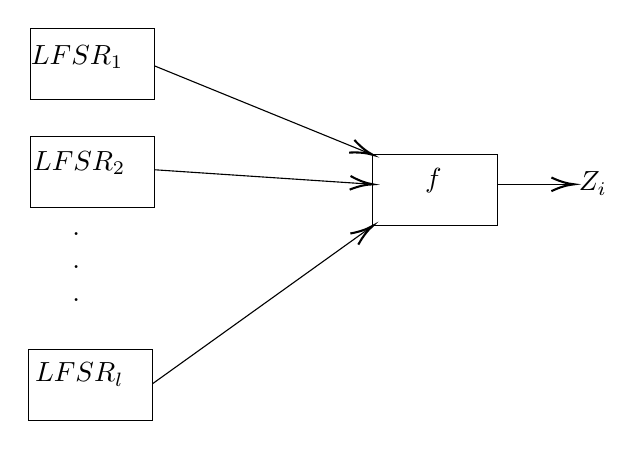
\begin{tikzpicture}[x=0.75pt,y=0.75pt,yscale=-1,xscale=1]
        \draw   (121,47) -- (181,47) -- (181,81.2) -- (121,81.2) -- cycle ;
        \draw   (120,202) -- (180,202) -- (180,236.2) -- (120,236.2) -- cycle ;
        \draw   (121,99) -- (181,99) -- (181,133.2) -- (121,133.2) -- cycle ;
        \draw   (286,108) -- (346,108) -- (346,142.2) -- (286,142.2) -- cycle ;
        \draw    (181,65.2) -- (284.15,107.25) ;
        \draw [shift={(286,108)}, rotate = 202.18] [color={rgb, 255:red, 0; green, 0; blue, 0 }  ][line width=0.75]    (10.93,-3.29) .. controls (6.95,-1.4) and (3.31,-0.3) .. (0,0) .. controls (3.31,0.3) and (6.95,1.4) .. (10.93,3.29)   ;
        \draw    (181,115.2) -- (284,122.07) ;
        \draw [shift={(286,122.2)}, rotate = 183.81] [color={rgb, 255:red, 0; green, 0; blue, 0 }  ][line width=0.75]    (10.93,-3.29) .. controls (6.95,-1.4) and (3.31,-0.3) .. (0,0) .. controls (3.31,0.3) and (6.95,1.4) .. (10.93,3.29)   ;
        \draw    (180,218.2) -- (284.37,143.37) ;
        \draw [shift={(286,142.2)}, rotate = 144.36] [color={rgb, 255:red, 0; green, 0; blue, 0 }  ][line width=0.75]    (10.93,-3.29) .. controls (6.95,-1.4) and (3.31,-0.3) .. (0,0) .. controls (3.31,0.3) and (6.95,1.4) .. (10.93,3.29)   ;
        \draw    (346,122.2) -- (381,122.2) ;
        \draw [shift={(383,122.2)}, rotate = 180] [color={rgb, 255:red, 0; green, 0; blue, 0 }  ][line width=0.75]    (10.93,-3.29) .. controls (6.95,-1.4) and (3.31,-0.3) .. (0,0) .. controls (3.31,0.3) and (6.95,1.4) .. (10.93,3.29)   ;
        
        \draw (120,54) node [anchor=north west][inner sep=0.75pt]   [align=left] {$LFSR_1$};
        \draw (121,105) node [anchor=north west][inner sep=0.75pt]   [align=left] {$LFSR_2$};
        \draw (122,207) node [anchor=north west][inner sep=0.75pt]   [align=left] {$LFSR_l$};
        \draw (310,113) node [anchor=north west][inner sep=0.75pt]   [align=left] {$f$};
        \draw (140,144) node [anchor=north west][inner sep=0.75pt]   [align=left] {.\\.\\.};
        \draw (384,115) node [anchor=north west][inner sep=0.75pt]   [align=left] {$Z_i$};
    \end{tikzpicture}\\
    $C_i = m_i \oplus Z_i$
\end{center}    

\textbf{Example:} Consider the following 3-LFSR with non-liner filter function $f$.
\begin{center}
    \tikzset{every picture/.style={line width=0.75pt}}       
    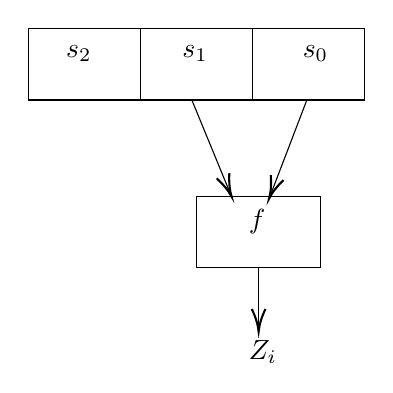
\begin{tikzpicture}[x=0.75pt,y=0.75pt,yscale=-1,xscale=1]
        \draw   (444,57) -- (498,57) -- (498,91.6) -- (444,91.6) -- cycle ;
        \draw   (498,57) -- (552,57) -- (552,91.6) -- (498,91.6) -- cycle ;
        \draw   (552,57) -- (606,57) -- (606,91.6) -- (552,91.6) -- cycle ;
        \draw   (525,138) -- (585,138) -- (585,172.2) -- (525,172.2) -- cycle ;
        \draw    (523,92) -- (541.24,136.35) ;
        \draw [shift={(542,138.2)}, rotate = 247.64] [color={rgb, 255:red, 0; green, 0; blue, 0 }  ][line width=0.75]    (10.93,-3.29) .. controls (6.95,-1.4) and (3.31,-0.3) .. (0,0) .. controls (3.31,0.3) and (6.95,1.4) .. (10.93,3.29)   ;
        \draw    (578,92.2) -- (560.72,137.33) ;
        \draw [shift={(560,139.2)}, rotate = 290.96] [color={rgb, 255:red, 0; green, 0; blue, 0 }  ][line width=0.75]    (10.93,-3.29) .. controls (6.95,-1.4) and (3.31,-0.3) .. (0,0) .. controls (3.31,0.3) and (6.95,1.4) .. (10.93,3.29)   ;
        \draw    (555,172) -- (555,201.2) ;
        \draw [shift={(555,203.2)}, rotate = 270] [color={rgb, 255:red, 0; green, 0; blue, 0 }  ][line width=0.75]    (10.93,-3.29) .. controls (6.95,-1.4) and (3.31,-0.3) .. (0,0) .. controls (3.31,0.3) and (6.95,1.4) .. (10.93,3.29)   ;
        
        \draw (517,64) node [anchor=north west][inner sep=0.75pt]   [align=left] {$s_1$};
        \draw (461,64) node [anchor=north west][inner sep=0.75pt]   [align=left] {$s_2$};
        \draw (575,64) node [anchor=north west][inner sep=0.75pt]   [align=left] {$s_0$};
        \draw (549,143) node [anchor=north west][inner sep=0.75pt]   [align=left] {$f$};
        \draw (549,206) node [anchor=north west][inner sep=0.75pt]   [align=left] {$Z_i$};
    \end{tikzpicture}\\
    $f: \{0,1\}^2 \rightarrow \{0,1\}$\\
    $f(x_0, x_1) = x_0 \cdot x_1$
\end{center}
Here, if we draw the truth table of $f$, it will look like,

\begin{table}[h]
\centering
  \begin{tabular}{c|c||c}
        \textbf{$x_0$} & \textbf{$x_1$} & \textbf{$f$} \\
        \hline
        0 & 0 & 0 \\
        0 & 1 & 0 \\
        1 & 0 & 0 \\
        1 & 1 & 1 \\
  \end{tabular}
\end{table}
We can see that $Pr[Z = 0] = \frac{3}{4}$. Here, $f$ is not a good function because $Pr[Z = 0] > Pr[Z = 1]$, that is, it is highly biased. We need to design $f$ such that the output is unpredictable. Here, we can predict that output will be zero with a higher probability. If we have a stream cipher with this model and we are able to find out the $f$ function. We can eventually break the stream cipher. Therefore, $f$ must be selected carefully.

\subsection{Non-Linear Feedback Shift Register}
After a period of time, it became evident that while Linear Feedback Shift Registers (LFSRs) were effective ciphers, many encryption methods could still be compromised through various cryptanalysis techniques. To address this vulnerability, a new concept emerged in stream ciphers known as Non-Linear Feedback Shift Registers (NFSRs). As the name implies, NFSRs incorporate a non-linear feedback function, distinguishing them from LFSRs. In contemporary cryptography, NFSRs serve as the foundation for most stream ciphers.

Unlike LFSRs, where the feedback function is linear, NFSRs introduce non-linearity into the feedback mechanism. However, one challenge with NFSRs is the absence of a systematic method for determining their period. In LFSRs, if the connection polynomial is primitive, the register achieves full periodicity. Conversely, in NFSRs, no such proof or methodology exists to determine their period.




\section{Hash Function}
It is a mapping from one set to another set.\\
\begin{center}
    $h : A \rightarrow B$\\
    $h(X) = Y$
\end{center}
Every hash function has following properties:
\begin{enumerate}
    \item If X is altered to $X'$, then h($X'$) will be completely different from h(X).
    \item Given Y, it is practically infeasible to find X s.t. h(X) = Y.
    \item Given X and Y = h(X), it is practically infeasible to find $X'$ s.t. h(X) = h($X'$).
\end{enumerate}
Let us consider this scenario where Alice is encrypting some message using symmetric key and sending it to Bob. 
\begin{center}
    

\tikzset{every picture/.style={line width=0.75pt}} %set default line width to 0.75pt        

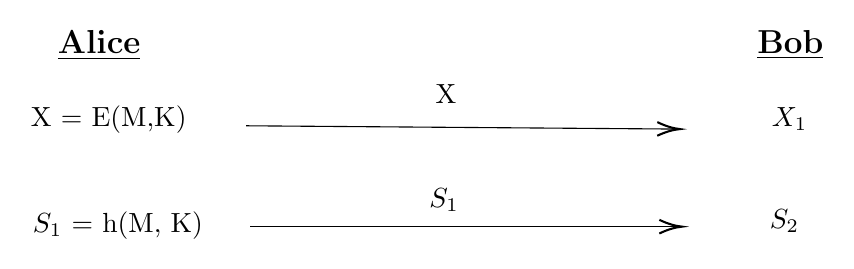
\begin{tikzpicture}[x=0.75pt,y=0.75pt,yscale=-1,xscale=1]
%uncomment if require: \path (0,300); %set diagram left start at 0, and has height of 300

%Straight Lines [id:da6936070700935975] 
\draw    (247,132) -- (454,133.58) ;
\draw [shift={(456,133.6)}, rotate = 180.44] [color={rgb, 255:red, 0; green, 0; blue, 0 }  ][line width=0.75]    (10.93,-3.29) .. controls (6.95,-1.4) and (3.31,-0.3) .. (0,0) .. controls (3.31,0.3) and (6.95,1.4) .. (10.93,3.29)   ;
%Straight Lines [id:da1977592175436449] 
\draw    (249,180.6) -- (455,180.6) ;
\draw [shift={(457,180.6)}, rotate = 180] [color={rgb, 255:red, 0; green, 0; blue, 0 }  ][line width=0.75]    (10.93,-3.29) .. controls (6.95,-1.4) and (3.31,-0.3) .. (0,0) .. controls (3.31,0.3) and (6.95,1.4) .. (10.93,3.29)   ;

% Text Node
\draw (155,85) node [anchor=north west][inner sep=0.75pt]   [align=left] {\textbf{{\large \underline{Alice}}}};
% Text Node
\draw (492,85) node [anchor=north west][inner sep=0.75pt]   [align=left] {\textbf{\underline{{\large Bob}}}};
% Text Node
\draw (142,121) node [anchor=north west][inner sep=0.75pt]   [align=left] {X = E(M,K)};
% Text Node
\draw (499,122) node [anchor=north west][inner sep=0.75pt]   [align=left] {$X_1$};
% Text Node
\draw (143,172) node [anchor=north west][inner sep=0.75pt]   [align=left] {$S_1$ = h(M, K)};
% Text Node
\draw (498,171) node [anchor=north west][inner sep=0.75pt]   [align=left] {$S_2$};
% Text Node
\draw (337,111) node [anchor=north west][inner sep=0.75pt]   [align=left] {X};
% Text Node
\draw (334,161) node [anchor=north west][inner sep=0.75pt]   [align=left] {$S_1$};


\end{tikzpicture}

\end{center}

Now, we want to verify that the message is coming from Alice and it has not been altered. Suppose if Bob receives the altered cipher text
$\tilde{X}$. Then on decryption using key K, Bob will not get the message M. So we need to ensure that the cipher text is coming from Alice and has not been altered. For that we use hash function. \\
\begin{center}
    If h($X_1$, K) = $S_2$, then Bob accepts $X_1$.
\end{center}
Since for hash function, if the input is changed even slightly, there is huge change in output. So if $X_1$ would have been altered even on a single bit, the output will not satisfy. Also, since we know input $X_1$ and the output of h(M, K) = $S_2$, still because of the properties of hash function, we still cannot determine message m and it is secure.
This is known as the Message Authentication Code. We are able to verify :
\begin{itemize}
    \item Whether X is altered during communication
    \item Whether $S_1$ is altered during communication
\end{itemize}


\subsection*{Definition}
A hash family is defined as a four-tuple $(P, S, K, H)$ where the following conditions hold:
\begin{enumerate}
    \item $P$ represents the set of all possible messages.
    \item $S$ denotes the set of all possible message digests or authentication tags (all output).
    \item $K$ signifies the key space.
    \item For each $K_1 \in K$, there exists a hash function $h_{K_1}$ such that $h_{K_1} : P \rightarrow S$, where $|P| \geq |S|$, and notably, $|P| \geq 2 \times |S|$.
\end{enumerate}
\begin{center}
    

\tikzset{every picture/.style={line width=0.75pt}} %set default line width to 0.75pt        

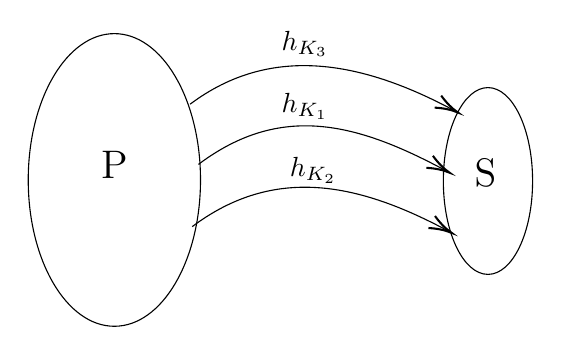
\begin{tikzpicture}[x=0.75pt,y=0.75pt,yscale=-1,xscale=1]
%uncomment if require: \path (0,300); %set diagram left start at 0, and has height of 300

%Shape: Ellipse [id:dp6385929644721748] 
\draw   (130.2,139.1) .. controls (130.2,100.16) and (148.78,68.6) .. (171.7,68.6) .. controls (194.62,68.6) and (213.2,100.16) .. (213.2,139.1) .. controls (213.2,178.04) and (194.62,209.6) .. (171.7,209.6) .. controls (148.78,209.6) and (130.2,178.04) .. (130.2,139.1) -- cycle ;
%Shape: Ellipse [id:dp35632658610404433] 
\draw   (330.2,139.6) .. controls (330.2,114.75) and (339.83,94.6) .. (351.7,94.6) .. controls (363.57,94.6) and (373.2,114.75) .. (373.2,139.6) .. controls (373.2,164.45) and (363.57,184.6) .. (351.7,184.6) .. controls (339.83,184.6) and (330.2,164.45) .. (330.2,139.6) -- cycle ;
%Curve Lines [id:da9831191387685083] 
\draw    (208.2,102.6) .. controls (247.8,72.9) and (292.3,82.4) .. (335.88,105.88) ;
\draw [shift={(337.2,106.6)}, rotate = 208.61] [color={rgb, 255:red, 0; green, 0; blue, 0 }  ][line width=0.75]    (10.93,-3.29) .. controls (6.95,-1.4) and (3.31,-0.3) .. (0,0) .. controls (3.31,0.3) and (6.95,1.4) .. (10.93,3.29)   ;
%Curve Lines [id:da7449905549695661] 
\draw    (212.2,131.6) .. controls (251.8,101.9) and (288.46,111.4) .. (331.88,134.88) ;
\draw [shift={(333.2,135.6)}, rotate = 208.61] [color={rgb, 255:red, 0; green, 0; blue, 0 }  ][line width=0.75]    (10.93,-3.29) .. controls (6.95,-1.4) and (3.31,-0.3) .. (0,0) .. controls (3.31,0.3) and (6.95,1.4) .. (10.93,3.29)   ;
%Curve Lines [id:da6241272700976574] 
\draw    (209.2,161.6) .. controls (248.8,131.9) and (289.38,140.42) .. (332.88,163.88) ;
\draw [shift={(334.2,164.6)}, rotate = 208.61] [color={rgb, 255:red, 0; green, 0; blue, 0 }  ][line width=0.75]    (10.93,-3.29) .. controls (6.95,-1.4) and (3.31,-0.3) .. (0,0) .. controls (3.31,0.3) and (6.95,1.4) .. (10.93,3.29)   ;

% Text Node
\draw (164,124) node [anchor=north west][inner sep=0.75pt]   [align=left] {{\Large P}};
% Text Node
\draw (344,128) node [anchor=north west][inner sep=0.75pt]   [align=left] {{\Large S}};
% Text Node
\draw (251,66) node [anchor=north west][inner sep=0.75pt]   [align=left] {$h_{K_3}$};
% Text Node
\draw (251,96) node [anchor=north west][inner sep=0.75pt]   [align=left] {$h_{K_1}$};
% Text Node
\draw (255,127) node [anchor=north west][inner sep=0.75pt]   [align=left] {$h_{K_2}$};


\end{tikzpicture}

Where H : set of all hash function
$h_{k_i}$ : hash function
\end{center}
\vspace{3mm}
\subsection{Types of Hash Function}
\begin{itemize}
    \item \textbf{Keyed Hash function : } In these hash functions, key is involved in the computation of hash value.
    \item \textbf{Unkeyed Hash function : } In these hash functions, key is not required to compute the hashed value.
\end{itemize}

\subsection{Problems}
\textbf{Problem 1:}\\
\begin{center}
    h : $ P \rightarrow S$
\end{center}
Given $y \in S$, find $x \in P$ such that h(x) = y. \\
\newline
This problem is known as the 'preimage finding problem'. For a hash function, h if you cannot find preimage in feasible time, then h is known as preimage resistant hash function. It is computationally difficult to find preimage for such functions.The preimage finding problem involves finding a specific input $x$ in the domain $P$ such that its hash value $h(x)$ equals a given value $y$ in the codomain $S$. Formally, given $y \in S$, the objective is to find $x \in P$ such that $h(x) = y$. This challenge is significant in hash function analysis, as it determines the resistance of the hash function against preimage attacks. A hash function is considered preimage resistant if it is computationally infeasible to find a preimage $x$ for a given hash value $y$ within a reasonable amount of time.\\
\newline
\textbf{Problem 2:}\\
\begin{center}
    h : $ P \rightarrow S$
\end{center}
Given $x \in p$ and h(x), find $x' \in P$ such that $x' \neq x$ and $h(x') = h(x)$.\\
\newline
This problem is known as 'Second preimage finding problem'. If finding second preimage is computationally hard for h, then it is known as second preimage resistant hash function.The second preimage finding problem entails finding a distinct input $x'$ in the domain $P$ such that its hash value $h(x')$ matches the hash value $h(x)$ of a given input $x$. Specifically, for a hash function $h : P \rightarrow S$, given an input $x$ and its hash value $h(x)$, the goal is to find another input $x'$ such that $x' \neq x$ and $h(x') = h(x)$. If it is computationally challenging to find such a second preimage for a given input, then the hash function is considered second preimage resistant.\\
\newline
\textbf{Problem 3:}\\
\begin{center}
    h : $ P \rightarrow S$
\end{center}
Find x, $x' \in P$ such that $x \neq x'$ and $h(x) = h(x')$\\
\newline
Additionally, in hash function analysis, another critical problem arises, known as the collision finding problem. This issue pertains to the identification of two distinct inputs \( x \) and \( x' \) in the domain \( P \) that produce the same hash value \( h(x) = h(x') \). A hash function \( h \) is considered collision-resistant if finding such collisions is computationally challenging.

\subsection{Ideal Hash Function}
An ideal hash function, denoted as \( h : P \rightarrow S \), is characterized by a unique property. It ensures that given an input \( x \in P \), obtaining its hash value \( h(x) \) can only be achieved through two methods: directly applying the hash function to \( x \) or consulting the hash table where \( h(x) \) is stored. This exclusive characteristic defines the ideal nature of the hash function.


\subsection{Pre image finding algorithm}
\begin{center}
    h : $X \rightarrow Y$
\end{center}
$|Y|=M$\\
Choose any $X_o \subseteq X$ such that $|X_o| = Q$\\
\begin{center}
\tikzset{every picture/.style={line width=0.75pt}} %set default line width to 0.75pt        

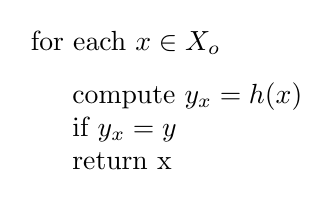
\begin{tikzpicture}[x=0.75pt,y=0.75pt,yscale=-1,xscale=1]
%uncomment if require: \path (0,300); %set diagram left start at 0, and has height of 300


% Text Node
\draw (114,67) node [anchor=north west][inner sep=0.75pt]   [align=left] {for each $x \in X_o$};
% Text Node
\draw (134,92) node [anchor=north west][inner sep=0.75pt]   [align=left] {compute $y_x = h(x)$
\\if $y_x = y$
\\ return x};


\end{tikzpicture}

\end{center}
The chance of getting pre-image depends on the selection of $X_o$. \\
\newline
Let us find the probability of finding pre-image using $X_o$\\
\begin{center}
    $X_o = \{x_1, x_2, \dots , x_Q \}$\\
    $E_i : event h(x_i) = y; 1 \leq i \leq Q$
\end{center}
h(x) can have M values, out of which only one will give success. So,
\begin{center}
    $Pr[E_i] = \frac{1}{M}$\\
    $Pr[{E_i}'] = 1- \frac{1}{M}$
\end{center}
Now we accumulate the probabilities of $E_1, E_2 \dots E_Q$
\begin{center}
    $Pr[E_1 \cup E_2 \cup E_3 \cup \dots \cup E_Q] = 1 - Pr[{E_1}' \cap {E_2}' \cap {E_3}' \cap \dots \cap {E_Q}']$\\
    \vspace{3mm}
    $Pr[E_1 \cup E_2 \cup E_3 \cup \dots \cup E_Q] = 1 - \prod_{i=1}^{Q} Pr[{E_i}']$\\
    \vspace{3mm}
    $Pr[E_1 \cup E_2 \cup E_3 \cup \dots \cup E_Q] = 1 - {(1-\frac{1}{M})}^Q$
\end{center}
Let us expand it now. 
\begin{center}
    $Pr[E_1 \cup E_2 \cup E_3 \cup \dots \cup E_Q] = 1 - [1-(\binom{Q}{1} \frac{1}{M} + \binom{Q}{2} \frac{1}{M^2} \dots]$\\
    \vspace{3mm}
    $Pr[E_1 \cup E_2 \cup E_3 \cup \dots \cup E_Q] \approx  1 - [1-(\binom{Q}{1} \frac{1}{M}]$\\
    \vspace{3mm}
    $Pr[E_1 \cup E_2 \cup E_3 \cup \dots \cup E_Q] \approx \frac{Q}{M}$
\end{center}
Therefore, 
\begin{center}
    Pr[ pre image finding ] = $\frac{Q}{M}$\\
    \vspace{3mm}
    Complexity(pre image finding) = O(M)
\end{center}
\end{document}

\end{document}